\documentclass[12pt]{article}
\usepackage[a4paper, margin=1in]{geometry}
\usepackage{graphicx} % 插入图片
\usepackage{float}    % 控制浮动体
\usepackage{hyperref} % 添加超链接
\usepackage{booktabs} % 提供更美观的表格线
\usepackage{amsmath}  % 数学公式支持
\usepackage{array}    % 表格增强
\usepackage{caption}  % 图表标题设置
\captionsetup{font=small, labelfont=bf}
\renewcommand{\baselinestretch}{1.2} % 调整行间距
\begin{document}

\begin{figure}
    
\includegraphics[width=0.4\textwidth]{./src/logo2.png}
    \hfill
    \includegraphics[width=0.4\textwidth]{./src/Université_Paris_Saclay_-_logo.png}
\end{figure}

\title{CNN Practical with Cifar10}
\author{Jiahong Geng}
\date{\today}




\maketitle
\tableofcontents
\newpage
\section{Introduction}
The CIFAR-10 dataset (Canadian Institute For Advanced Research) is a collection of images that are commonly used to train machine learning and computer vision algorithms.
It is one of the most widely used datasets for machine learning research.
The CIFAR-10 dataset contains 60,000 32x32 color images in 10 different classes (airplanes, cars, birds, cats, deer, dogs, frogs, horses, ships, and trucks). There are 6,000 images of each class.
\begin{figure}[H]
    \centering
    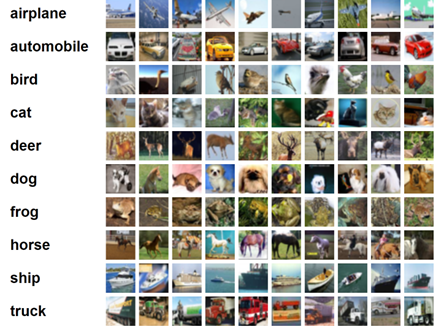
\includegraphics[width=0.5\textwidth]{./src/cifar10.png}
    \caption{CIFAR-10 Exemple}
\end{figure}
In the first part of this practical, I implemented a simple Convolutional Neural Network (CNN) to classify images from the CIFAR-10 dataset. 

In the second part of this practical, I implemented a Vision Transformer (ViT) to classify images from the CIFAR-10 dataset. 
The goal is to achieve better accuracy.
\section{Convolutional Neural Network(CNN)}
\subsection{Model Architecture}
The architecture of the CNN model is as follows:
\begin{table}[H]
    \centering
    \begin{tabular}{c|c|c}
        \hline
        Layer (type) & Input Shape & Output Shape \\
        \hline
        Conv2D & (None, 32, 32, 3) & (None, 30, 30, 32) \\
        MaxPooling2D & (None, 30, 30, 32) & (None, 15, 15, 32) \\
        Conv2D & (None, 15, 15, 32) & (None, 13, 13, 64) \\
        MaxPooling2D & (None, 13, 13, 64) & (None, 6, 6, 64) \\
        Conv2D & (None, 6, 6, 64) & (None, 4, 4, 64) \\
        Flatten & (None, 4, 4, 64) & (None, 1024) \\
        Dense & (None, 1024) & (None, 64) \\
        Dense & (None, 64) & (None, 10) \\
        \hline
    \end{tabular}
    \caption{CNN Model Architecture}
\end{table}
\subsection{Dataset Preprocessing and Model Training}
The CIFAR-10 dataset was loaded using the Keras library. 
The images were normalized and the labels were one-hot encoded.
The model was trained using the Adam optimizer and the categorical cross-entropy loss function. 
The model was trained for 10 epochs.
\subsection{Results}
The model achieved accuracy of 71.55\% on the test set after 10 epochs of training. 
The training and validation accuracy curves are shown below:
\begin{figure}[H]
    \centering
    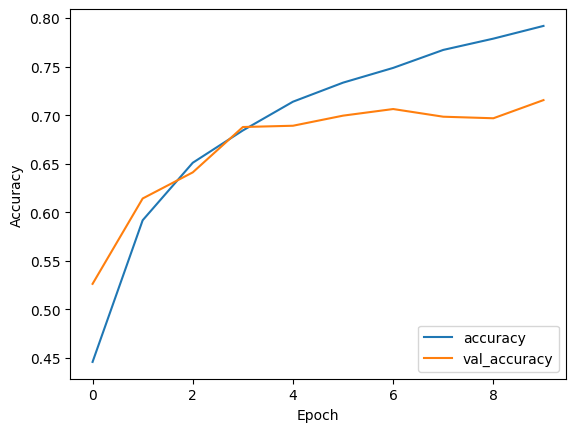
\includegraphics[width=0.4\textwidth]{./src/cnn_accuracy.png}
    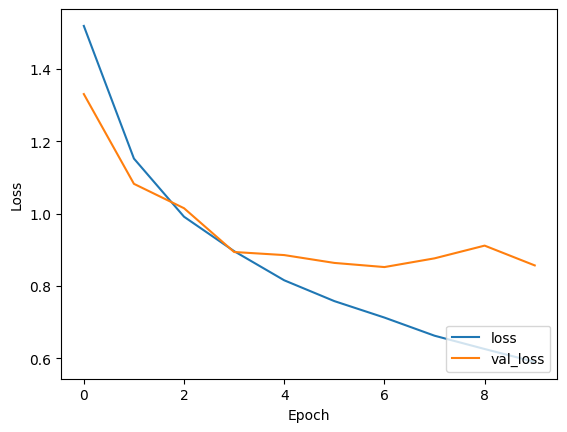
\includegraphics[width=0.4\textwidth]{./src/cnn_loss.png}
    \caption{CNN Accuracy and Loss Curves}
\end{figure}
The figure shows how the accuracy of the model changes with the number of training rounds (epochs) during training. 
The chart contains two curves: one represents the accuracy of the training set (accuracy) and the other represents the accuracy of the validation set (val\_accuracy).

The result metrics are shown in the table below:
\begin{table}[H]
    \centering
    \begin{tabular}{c|c}
        \hline
        Metric & Value \\
        \hline
        Best Training Accuracy & 79.19\% \\
        Best Validation Accuracy & 71.55\% \\
        Test Accuracy & 71.55\% \\
        Best Training Loss & 0.58994 \\
        Best Validation Loss & 0.85235 \\
        Test Loss & 0.85692 \\
        \hline
    \end{tabular}
    \caption{CNN Training, Validation, and Test Metrics}
\end{table}
\subsection{Parsing the Output}
The output of the model is a probability distribution over the 10 classes. 
The array below shows the predicted probabilities for each class for a single image:

\begin{verbatim}
array([[4.7004773e-04, 1.1618343e-03, 2.1541063e-03, 3.1325072e-02,
        2.0603200e-03, 9.6137750e-01, 7.0366100e-04, 9.1952134e-05,
        5.1872976e-06, 6.5037055e-04]], dtype=float32)
\end{verbatim}

The class with the highest probability is the predicted class. 
In this case, the model predicts the class with the highest probability as the class corresponding to the index with the value 0.65835053.
\subsection{Layer Visualization}
I visualized the feature maps of the first five layers of this CNN model. 
Feature maps show the features extracted by the model at different levels.

The first layer is Conv2D layers, which are used to extract features from the input image. 
The feature maps of the first layer show the edges and textures of the input image.
The second layer is MaxPooling2D layers, which are used to downsample the feature maps. 
The feature maps of the second layer show the downsampled features of the input image.
The feature maps of the first and second layers are shown below:
\begin{figure}[H]
    \centering
    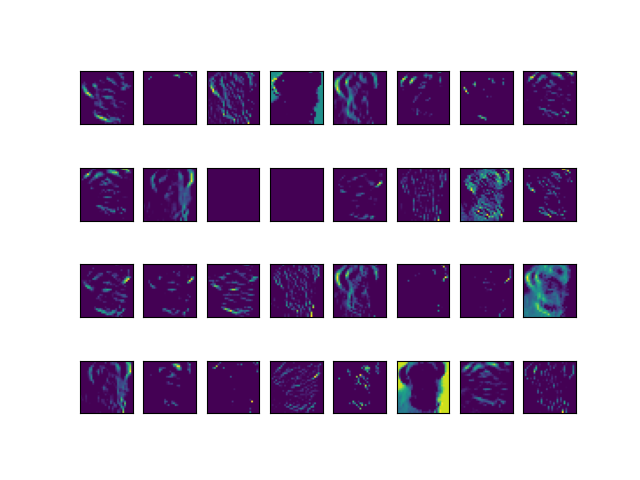
\includegraphics[width=0.4\textwidth]{./src/cnn_layer_1.png}
    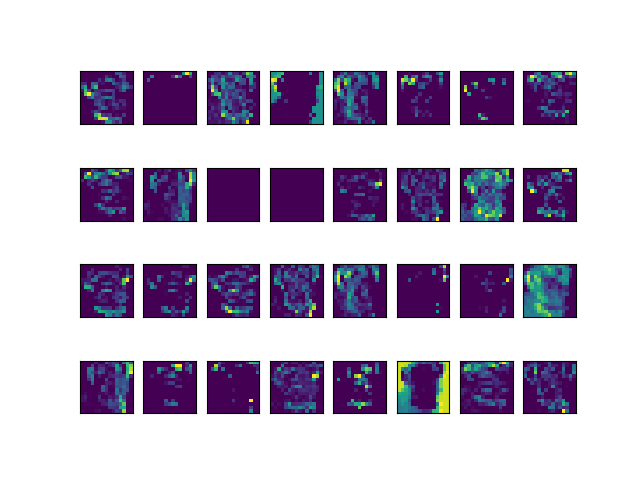
\includegraphics[width=0.4\textwidth]{./src/cnn_layer_2.png}
    \caption{CNN Layer 1 and 2 Feature Maps}
\end{figure}
The third layer extracts more complex features, the fourth layer downsamples these features, and the fifth layer extracts even more complex features. 
The feature maps of these layers are shown below:
\begin{figure}[H]
    \centering
    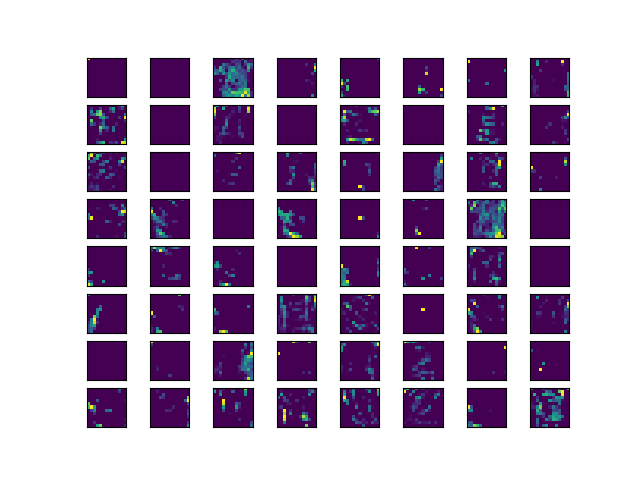
\includegraphics[width=0.3\textwidth]{./src/cnn_layer_3.png}
    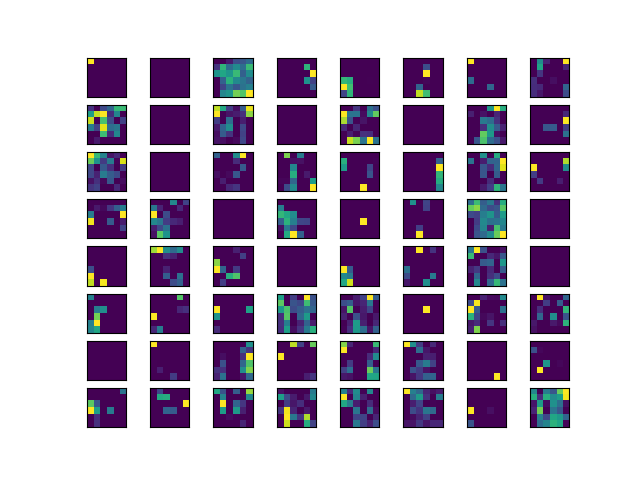
\includegraphics[width=0.3\textwidth]{./src/cnn_layer_4.png}
    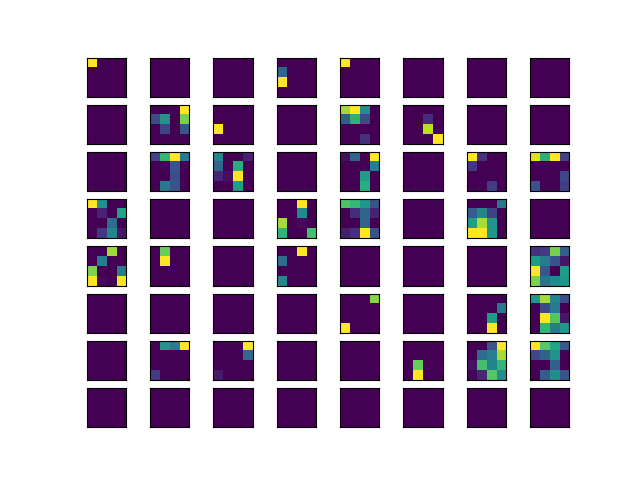
\includegraphics[width=0.3\textwidth]{./src/cnn_layer_5.png}
    \caption{CNN Layer 3, 4, and 5 Feature Maps}
\end{figure}
\subsection{Results of 200 epochs}
The accuracy and loss curves after 200 epochs are shown below:
\begin{figure}[H]
    \centering
    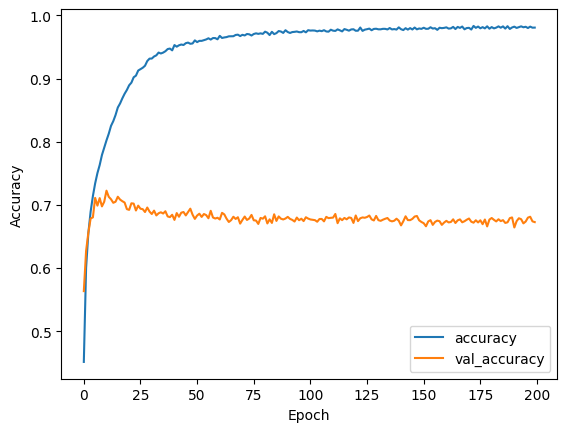
\includegraphics[width=0.49\textwidth]{./src/cnn_accuracy_200.png}
    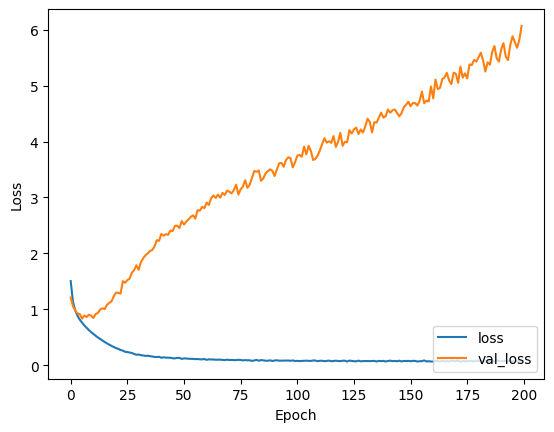
\includegraphics[width=0.49\textwidth]{./src/cnn_loss_200.png}
    \caption{CNN Accuracy and Loss Curves (200 epochs)}
\end{figure}
The result metrics are shown in the table below:
\begin{table}[H]
    \centering
    \begin{tabular}{c|c}
         \hline
            Metric & Value \\
            \hline
            Best Training Accuracy & 98.35\% \\
            Best Validation Accuracy & 72.25\% \\
            Test Accuracy & 67.27\% \\
            Best Training Loss & 0.05855 \\
            Best Validation Loss & 0.83243 \\
            Test Loss & 6.06786 \\
            \hline
    \end{tabular}
    \caption{CNN Training, Validation, and Test Metrics (200 epochs)}
\end{table}
More training steps did not improve the performance of the model.
This shows the limitation of the model with small parameters, which makes it difficult to capture more features.
The training of 200 epochs is mainly for comparison with the ViT model.
\subsection{Conclusion}
In this part of the practical, I implemented a Convolutional Neural Network (CNN) to classify images from the CIFAR-10 dataset.
The feature maps of the first five layers of the model show the features extracted at different levels of the network.
The model achieved accuracy of 71.55\% on the test set after 10 epochs of training and 67.27\% after 200 epochs.
The model did not show performance improvement and even showed signs of overfitting after more training, which indicates that the model has reached its capacity limit for the given dataset. 
This suggests that the model is too simple to capture more complex features from the data, and increasing the training epochs only leads to the model memorizing the training data rather than generalizing well to unseen data. 
This highlights the need for a more complex model or additional regularization techniques to improve performance.
\section{Vision Transformer(ViT)}
\subsection{Introduction}
The ViT is a deep learning model that uses the transformer architecture to process images. 
The ViT model has been shown to achieve state-of-the-art performance on image classification tasks. 
In this practical, I implemented a ViT to classify images from the CIFAR-10 dataset. 
The goal was to achieve better accuracy than the Convolutional Neural Network (CNN) model implemented in the first part of this practical.
\subsection{Model Architecture}
The ViT splits an input image of size $H \times W \times C$ into non-overlapping patches of size $P \times P$ and generates $N = \frac{HW}{P^2}$ patches. 
Each patch is flattened and projected into a $D$-dimensional embedding space. 
A learnable positional embedding is then added to the sequence (with a prepended classification token), which is processed through $L$ layers of transformer encoder blocks—each containing a multi-head self-attention mechanism and a feed-forward network with residual connections. 
The final classification is obtained by feeding the output corresponding to the classification token into an MLP head.
\begin{figure}[H]
    \centering
    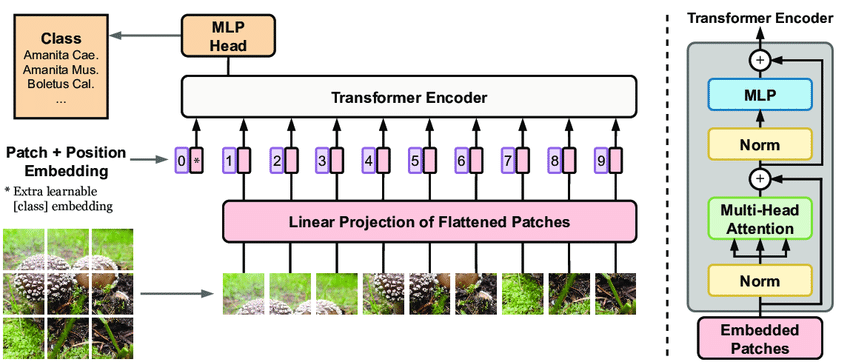
\includegraphics[width=0.8\textwidth]{./src/vit.png}
    \caption{ViT Architecture}
\end{figure}
\subsection{Dataset Preprocessing and Model Training}
The dataset is first preprocessed by resizing images to a uniform resolution and normalizing pixel values. 
Data augmentation techniques, including random cropping and horizontal flipping, are applied to improve generalization. 
The vision transformer model is trained using the Adam optimizer with an initial learning rate scheduled to decay over time. 
Training is conducted for a fixed number of epochs with a designated batch size, using cross-entropy loss as the objective function. 
Regularization methods such as dropout and early stopping are also employed to mitigate overfitting.
\subsection{Results}
The validation accuracy and loss curves after 200 epochs of training are shown below:
\begin{figure}[H]
    \centering
    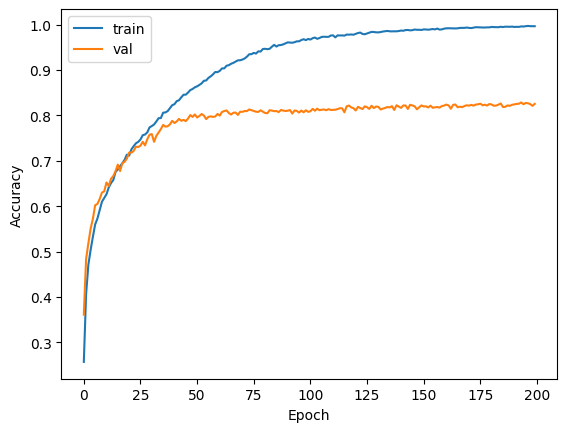
\includegraphics[width=0.4\textwidth]{./src/vit_acc.png}
    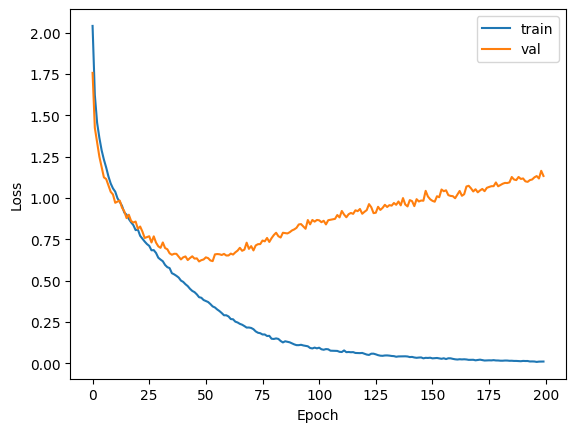
\includegraphics[width=0.4\textwidth]{./src/vit_loss.png}
    \caption{ViT Accuracy and Loss}
\end{figure}
The result of the model is shown in the table below:
\begin{table}[H]
    \centering
    \begin{tabular}{c|c}
        \hline
        Metric & Value \\
        \hline
        Best Training Accuracy & 99.89\% \\
        Best Validation Accuracy & 83.82\% \\
        Test Accuracy & 83.47\% \\
        Best Training Loss & 0.00444 \\
        Best Validation Loss & 0.59438 \\
        Test Loss & 1.07644 \\
        \hline
    \end{tabular}
    \caption{ViT Training, Validation, and Test Metrics}
\end{table}
\subsection{Compare with CNN}
The ViT model achieved accuracy of 83.47\% on the test set after 200 epochs. 
This is a significant improvement over the CNN model, which achieved accuracy of 71.55\% on the test set after 200 epochs of training. 
The ViT model can capture more complex features and learn more effectively from the data, resulting in better performance on the image classification task.

The training and validation accuracy curves indicate that the ViT model is learning effectively and does not overfit the training data.
The ViT model can generalize well to unseen data and achieve higher accuracy on the test set.
\subsection{Pretrained Model}
Pre-trained models are trained on a larger dataset (e.g., ImageNet) and then fine-tuned on a smaller dataset (e.g., CIFAR-10). 
This allows the model to learn more general features from the larger dataset and then adapt to the specific characteristics of the smaller dataset.

The pre-trained model can achieve accuracy of 99.5\% on the test set. 
This is a significant improvement over the model trained from scratch, which achieved accuracy of 83.65\% on the test set. 
The pre-trained model can leverage the knowledge learned from the larger dataset to achieve better performance on the smaller dataset. 
This suggests that a larger number of parameters can be better utilized by training on a larger dataset.
\subsection{Conclusion}
In this part of the practical, I implemented a ViT to classify images from the CIFAR-10 dataset. 
The model achieved accuracy of 83.47\% on the test set after 200 epochs of training. 
The training and validation accuracy curves show that the ViT model is learning effectively and not overfitting the training data. 
The ViT model can capture more complex features and learn more effectively from the data, resulting in better performance on the image classification task.
\section{Summary}
In this practical, I implemented a CNN and a ViT to classify images from the CIFAR-10 dataset. 
The CNN model achieved an accuracy of 71.55\% on the test set after 10 epochs and 67.27\% after 200 epochs. 
More training did not improve performance, showing the limitations of the CNN model as a baseline. 
The ViT model achieved an accuracy of 83.47\% on the test set after 200 epochs, with accuracy curves indicating potential for further improvement. 
Research suggests that the ViT model trained directly on the CIFAR-10 dataset can achieve around 90\% accuracy.

Based on these results, we can conclude that the ViT model outperforms the CNN model, demonstrating the effectiveness of the Transformer architecture for image classification tasks. 
However, this is not the limit of the Transformer architecture. 
Currently, the ViT model pre-trained on the ImageNet-21K dataset is leading the CIFAR-10 contest with an accuracy of 99.5\%.
\section{Source Code}
The source code for this practical can be found on GitHub at the following link:
\url{https://github.com/JeffersonGeng/AI-CIFAR}
\end{document}